\documentclass[a4paper, 12pt, twoside]{article}
\usepackage[T2A,T1]{fontenc}
\usepackage[utf8]{inputenc}
\usepackage[english, russian]{babel}
\usepackage{graphicx}
\usepackage{ amssymb }
\usepackage[hcentering, bindingoffset = 10mm, right = 15 mm, left = 15 mm, top=20mm, bottom = 20 mm]{geometry}
\usepackage{multirow}
\usepackage{lipsum}
\usepackage{amsmath, amstext}
\usepackage{siunitx}
\usepackage{subcaption}
\usepackage{wrapfig}
\usepackage{adjustbox}
\usepackage{enumerate, indentfirst, float}
\usepackage{capt-of, svg}
\usepackage{ctable}
\usepackage{cmap} % Улучшенный поиск русских слов в полученном pdf-файле
\newcommand*{\hm}[1]{#1\nobreak\discretionary{} 
	{\hbox{$\mathsurround=0pt #1$}}{}}

\usepackage{pscyr} % Нормальные шрифты
\usepackage[normalem]{ulem} % для подчёркиваний uline
\ULdepth = 0.16em

\usepackage{fancyhdr} %Колонтикулы
\pagestyle{fancy}
\lhead{
\includegraphics[width = 10 mm]{logo.jpg} Лабораторная работа № 3.2.6}
\rhead{\textit{\today}}

\newenvironment{bottompar}{\par\vspace*{\fill}}{\clearpage}
 
\begin{document}
\begin{titlepage}

\newcommand{\HRule}{\rule{\linewidth}{0.7mm}} % Defines a new command for the horizontal lines, change thickness here

\center % Center everything on the page
 
%----------------------------------------------------------------------------------------
%	HEADING SECTIONS
%----------------------------------------------------------------------------------------

\textsc{\LARGE Московский Физико-Технический Институт}\\[1,5cm] % Name of your university/college
\textsc{\Large Кафедра общей физики}\\[0.5cm] % Major heading such as course name
\textsc{\large Лабораторная работа \textnumero  3.2.6}\\[0.5cm] % Minor heading such as course title

%----------------------------------------------------------------------------------------
%	TITLE SECTION
%----------------------------------------------------------------------------------------

\HRule
\\[0.4cm]
{ \huge \bfseries Исследование гальванометра.}
\\[0.2cm] % Title of your document
\HRule
\\[1.5cm]


 
%----------------------------------------------------------------------------------------
%	AUTHOR SECTION
%----------------------------------------------------------------------------------------

\begin{minipage}{0.4\textwidth}
	\begin{flushleft} \large
		\textbf{Автор:}\\
		Глеб Уваркин \\
		615 группа
	\end{flushleft}
\end{minipage}
~
\begin{minipage}{0.4\textwidth}
	\begin{flushright} \large
		\textbf {Преподаватель:} \\
		Андрей Александрович Заболотных % Supervisor's Name
	\end{flushright}
\end{minipage}

\begin{bottompar}
	\begin{center}
		
\includegraphics[width = 80 mm]{logo.jpg}
	\end{center}
	{\large \today}

\end{bottompar}
\vfill % Fill the rest of the page with whitespace

\end{titlepage}

{\Large \uline { \textbf  {Цель работы:}}}

\vspace{2mm}
Изучение работы высокочувствительного зеркального гальванометра магнитоэлектрической системы в режимах измерения постоянного тока и электрического заряда.
\vspace{\baselineskip}

{\Large \uline { \textbf  {В работе используются:}}}

\vspace{2mm}

Зеркальный гальванометр с осветителем и шкалой, источник постоянного напряжения, делитель напряжения, магазин сопротивлений, эталонный конденсатор, вольтметр, переключатель, ключи, линейка.

\section{Теоретические сведения.}


\begin{minipage}[l]{0.6\linewidth}
	\paragraph{Общее устройство.}
\textit{Баллистический гальванометр} -- электроизмерительный прибор магнитоэлектрической системы, отличающийся высокой чувствительностью к току и сравнительно большим периодом колебаний подвижной системы.
Два режима работы:
\begin{enumerate}
	\item[--] \textit{Стационарный} (измерение постоянного тока)
	\item[--] \textit{Баллистический} (измерение заряда, протекшего через рамку за некоторое время)
\end{enumerate}
\end{minipage}
~
\begin{minipage}[r]{0.3\linewidth}
\begin{figure}[H]
	\centering
	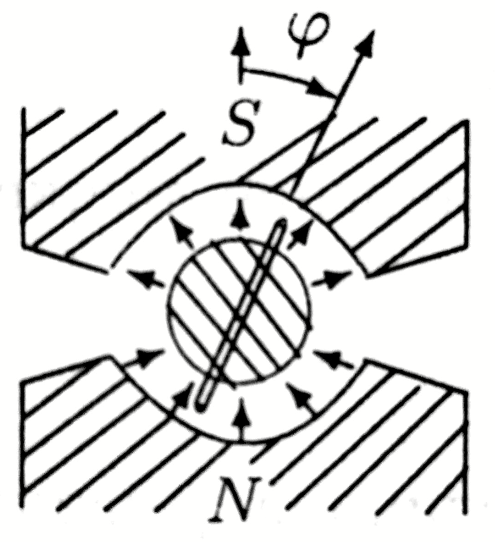
\includegraphics[width = 0.8\linewidth]{sch1}
	\caption[h]{Рамка с током в магнитном поле}
\end{figure}
\end{minipage}








\paragraph{Уравнение движения подвижной системы.}
Обозначим
\begin{equation}\label{eq:obz}
\left.
\begin{aligned}
\dfrac{(BSN)^2}{JR_\Sigma} = 2\gamma\\
\dfrac{D}{J} = \omega_0\\
\dfrac{BSN}{J} = K
\end{aligned}
\right\}
\end{equation}
Тогда уравнение движения рамки примет вид:
\begin{equation}\label{eq:urdv}
\ddot{\varphi} + 2\gamma\dot{\varphi} + \omega_0^2\gamma = KI,
\end{equation}
где $\gamma$ --\textit{ коэффициент затухания} подвижной системы гальванометра,\\ $\omega_0$ -- \textit{собственная частота} колебаний рамки

\paragraph{Режим измерения постоянного тока.}
При пропускании постоянного тока через рамку, то в уравнении \eqref{eq:urdv} можно положить $\ddot{\varphi} = \ddot{\varphi} = 0$ и угол поворота определится как:
\begin{equation}
\varphi = \dfrac{K}{\omega_0^2}I = \dfrac{I}{C_I},
\end{equation}
где $C_I$ -- \textit{динамическая постоянная} гальванометра.

\paragraph{Свободные колебания рамки.} Исследуем движение в отсутствие внешних источников тока, когда $I = 0$.

НУ:\hspace{10pt} при $t = 0$ \hspace{10pt} $\varphi = 0,$ \hspace{10pt} $\dot{\varphi} = \dot{\varphi_0}$.

Возможные случаи:
\begin{enumerate}
	\item $\gamma < \omega_0$ (колебательный режим).
	
	Решение задачи Коши однородного ур-ия для \eqref{eq:urdv} даст
	\begin{equation}
	\varphi = \dfrac{\dot{\varphi}_0}{\omega}e^{-\gamma t}\sin{\omega t},
	\end{equation}
	где 
	\begin{equation}\label{eq:omega}
	\omega^2 = \omega_0^2 - \gamma^2
	\end{equation}
	
	Движение рамки имеет колебательный характер и затухает со временем.
	
	Период таких колебаний равен:
	\begin{equation}
	T = \dfrac{2\pi}{\omega} = \dfrac{pi}{\sqrt{\frac{D}{J} - \frac{(BSN)^4}{(2JR_\Sigma)^2}}}
	\end{equation}
	
	Если затухание мало ($\gamma \ll \omega_0$), то движение рамки близко к синусоидальному
	\begin{equation}
	\varphi = \dfrac{\dot{\varphi}_0}{\omega_0}\sin{\omega_0 t}.
	\end{equation}
	
	\item $\gamma = \omega_0$ (критический режим).
	
	В этом случае
	\begin{equation}
	\varphi = \dot{\varphi}_0te^{-\gamma t}
	\end{equation}
	
	Движение не имеет колебательного характера: отклоненная подвижная система после отброса почти экспоненциально приближается к нулю.
	
	\item  $\gamma > \omega_0$ (случай переуспокоенного гальванометра).
	
	Решение все той же задачи примет вид
	\begin{equation}\label{eq:dphi}
	\varphi = \dfrac{\dot{\varphi}_0}{\varkappa}e^{-\gamma t}\sh{\varkappa t},
	\end{equation}
	где $$\varkappa^2 = \gamma^2 - \omega_0^2$$
	
	Движение остается апериодическим, однако подвижная система приближается к равновесию медленнее, чем в критическом режиме.
\end{enumerate} 

\paragraph{Режим измерения заряда}
При пропускании через рамку короткого импульса тока, можно считать, что весь ток успевает пройти при не отклоненном положении рамки, хотя она и получает толчок, в результате которого она приводится в движение, описываемое однородным уравнением \eqref{eq:urdv}, при заданных НУ.

Вычислим скорость $\dot{\varphi}_0$, при длительности импульса $\tau$:
\begin{equation}
\int_{0}^{\tau}\ddot{\varphi}dt + 2\gamma\int_{0}^{\tau}\dot{\varphi}dt + \omega_0^2\int_{0}^{\tau}\varphi dt = K\int_{0}^{\tau}Idt
\end{equation}
Второе и третье слагаемые малы, поэтому их мы не учитываем. Итого:
\begin{equation}
\dot{\varphi}(\tau) = Kq.
\end{equation}

Величину $C_Q = q/\varphi_{max}$ будем называть \textit{баллистической постоянной} гальванометра.

Максимальный отброс достигается при отсутствии затухания:
\begin{equation}
\varphi_{max\text{ св} } = \dfrac{\dot{\varphi}(\tau)}{\omega_0} = \dfrac{Kq}{\omega_0}
\end{equation}

В случае критического затухания
\begin{equation}
\varphi_{max\text{ кр} } = \dfrac{Kq}{\omega_0 e}
\end{equation}

Таким образом отношение баллистических постоянных для двух режимов:
\begin{equation}\nonumber
\dfrac{C_{Q\text{ кр}}}{C_{Q\text{ св}}} = e
\end{equation}

\subsection{Определение динамической постоянной}
\paragraph{Экспериментальная установка.}
\begin{figure}[H]
	\centering
	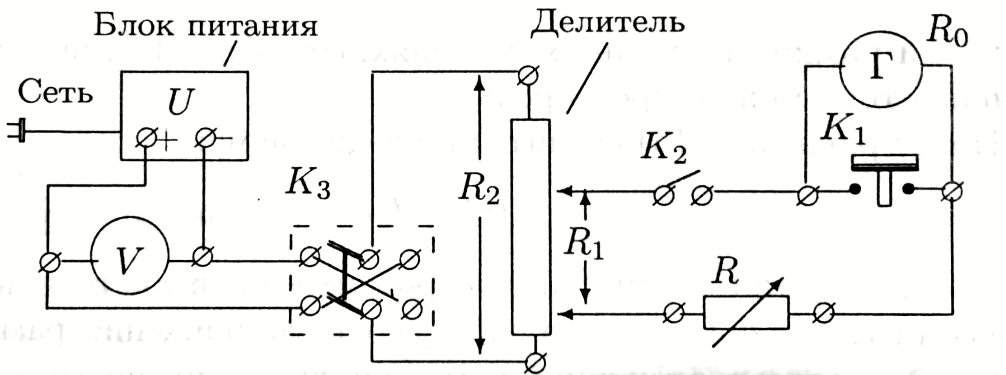
\includegraphics[width = 0.7\linewidth]{sch2}
	\caption{Схема установки для работы гальванометра в стационарном режиме}
	\label{sch:2}
\end{figure}
Схема установки представлена на Рис. \ref{sch:2}. При малых $R_1$ сила тока, протекающего через гальванометр может быть вычислена по очевидной формуле:

\begin{equation}
\label{f14}
I = U_0\dfrac{R_1}{R_2}\dfrac{1}{R + R_0},
\end{equation}

где $U_0$ -- показания вольтметра, $R_1/R_2$ -- положение делителя, $R$ -- сопротивление магазина, $R_0$ -- внутреннее сопротивление гальванометра.

Связь координаты $x$ светового пятна на шкале и углом отклонения рамки:
$$x = a\tg(2\varphi),$$
где $a$ -- расстояние от шкалы до зеркальца. При малых углах $\varphi = x/2a$. Динамическая постоянная
\begin{equation}
\label{f15}
C_I\left[\frac{\text{А}}{\text{мм/м}}\right] = \dfrac{I}{\varphi} = \dfrac{2aI}{x}.
\end{equation}

\subsection{Определение критического сопротивления гальванометра}
Схему будем использовать ту же.

При больших $R$ свободное движение рамки имеет колебательный характер. С его уменьшением увеличивается затухание и колебания переходят в апериодический режим.

Скорость затухания характеризуется \textit{логарифмическим декрементом затухания}

\begin{equation}\label{eq:theta}
\varTheta = \ln\dfrac{\varphi_n}{\varphi_{n+1}} = \ln\dfrac{x_n}{x_{n+1}} = \gamma T,
\end{equation}
где 

\begin{equation}\label{eq:T}
T = \dfrac{2\pi}{\omega}
\end{equation}

Измеряя зависимость $\varTheta(R)$ можно найти $R_\text{кр}$, при котором $\varTheta \rightarrow \infty$. Комбинируя формулы \eqref{eq:obz}, \eqref{eq:urdv}, \eqref{eq:omega}, \eqref{eq:theta} и \eqref{eq:T} получаем:
\begin{equation}
\varTheta = \dfrac{2\pi R_3}{\sqrt{(R + R_0)^2 - R_3^2}},
\end{equation}
где введено обозначение:
\begin{equation}
R_3 = \dfrac{(BSN)^2}{2\sqrt{JD}} = R_0 + R_{\text{кр}}
\end{equation}
Преобразовав предпоследнее выражение получим:
\begin{equation}
\dfrac{1}{\varTheta} = \dfrac{(R_0 + R)^2}{4\pi^2R_3^2} - \dfrac{1}{4\pi^2}
\end{equation}
Представив последнее на графике в осях $X = (R + R_0)^2, Y = 1/\varTheta^2$, получим прямую, угол наклона которой позволяет рассчитать критическое сопротивление
\begin{equation}
\label{f21}
R_{\text{кр}} = \dfrac{1}{2\pi}\sqrt{\dfrac{\Delta X}{\Delta Y}} - R_0.
\end{equation}

\subsection{Определение баллистической постоянной и критического сопротивления гальванометра, работающего в баллистическом режиме}
\begin{figure}[H]
	\centering
	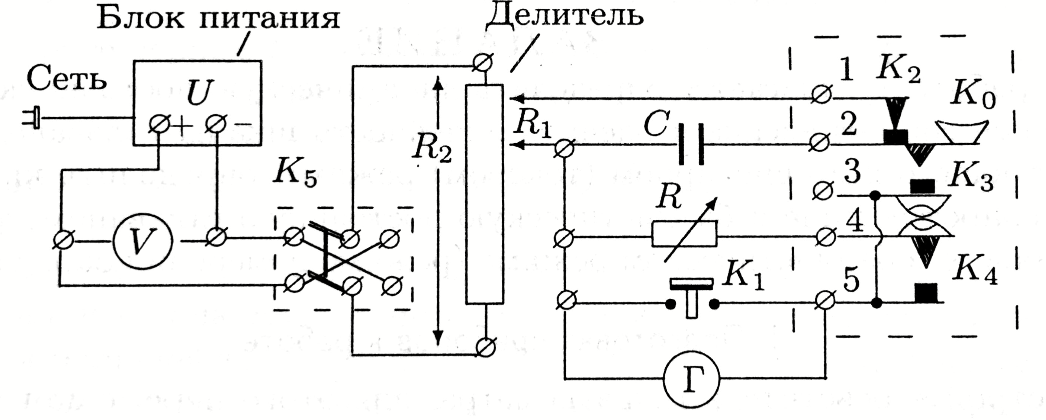
\includegraphics[width = 0.7\linewidth]{sch3}
	\caption{Схема установки для определения баллистической постоянной}
	\label{sch:3}
\end{figure}
Будем использовать схему, изображенную на Рис. \ref{sch:3}.

При нормальном положении кнопки $K_0$ конденсатор $C$ заряжается до напряжения
\begin{equation}\nonumber
U_C = \dfrac{R_1}{R_2}U_0.
\end{equation}
Заряд конденсатора равен
\begin{equation}
q = CU_C = \dfrac{R_1}{R_2}U_0C.
\end{equation}
Величину максимального отклонения гальванометра без затухания $\varphi_0$ можно рассчитать, если при разомкнутой цепи измерены максимальное отклонение рамки $\phi_1$ и логарифмический декремент затухания $\varTheta_0$.

Из ур-ий \eqref{eq:dphi} и \eqref{eq:theta}  следует, что при $\gamma \ll \omega_0$
\begin{equation}
\label{f23}
\varphi_0 = \varphi_1\cdot e^{\varTheta_0/4}
\end{equation}
Баллистическую постоянную гальванометра $C_{Q\text{ кр}}\left[\frac{\text{Кл}}{\text{мм/м}}\right]$ определяем при критическом сопротивлении:
\begin{equation}
\label{f24}
C_{Q\text{ кр}} = \dfrac{q}{\varphi_{max\text{ кр}}} = 2a\dfrac{R_1}{R_2}\dfrac{U_0C}{l_{max\text{ кр}}},
\end{equation}
где $l_{max\text{ кр}}$ --величина первого отброса в критическом режиме (мм), $а$ -- расстояние от зеркальца до шкалы (м), $U_0C$ -- заряд (Кл).
\newpage

\section{Обработка результатов.}
\subsection{Определение динамической постоянной.}
Снимем зависимость отклонения зайчика $x$ от сопротивления магазина $R$, увеличивая сопротивление магазина, но не меняя делителя ($U_0 = 1.38 \pm 0.02 ~\text{В},~ R_1/R_2 \simeq 1/2000,~R_2 = 10~\text{кОм},~R_0 = 280~\text{Ом},~2a = 2.2~\text{м}$). Рассчитаем токи $I$ по формуле (\ref{f14}) и построим график $I = f(x)$.
\begin{table}[H]
	\centering
	\caption{Зависимость I(x).}
	\label{t1}
	\begin{tabular}{c|cccccccccc}\toprule
		$R,~\text{кОм}$                  & 4.3  & 5.3  & 6.3  & 7.3  & 8.3  & 9.3  & 10.3 & 11.3 & 12.3 & 13.3 \\
		$x,~\text{см}$                   & 23.3 & 19   & 16   & 13.8 & 12.1 & 10.8 & 9.8  & 9    & 8.3  & 7.6  \\
		$I\cdot 10^{-8},~\text{А}$       & 15.1 & 12.4 & 10.5 & 9.1  & 8.0  & 7.2  & 6.5  & 5.9  & 5.5  & 5.1  \\ \midrule
		$\sigma_x,~\text{см}$            & \multicolumn{10}{c}{0.1}                                            \\
		$\sigma_I\cdot 10^{-9},~\text{А}$ & 3    & 2    & 2    & 2    & 2    & 1    & 1    & 1    & 1    & 1   \\ \bottomrule
	\end{tabular}
\end{table}
\begin{figure}[H]
	\centering
	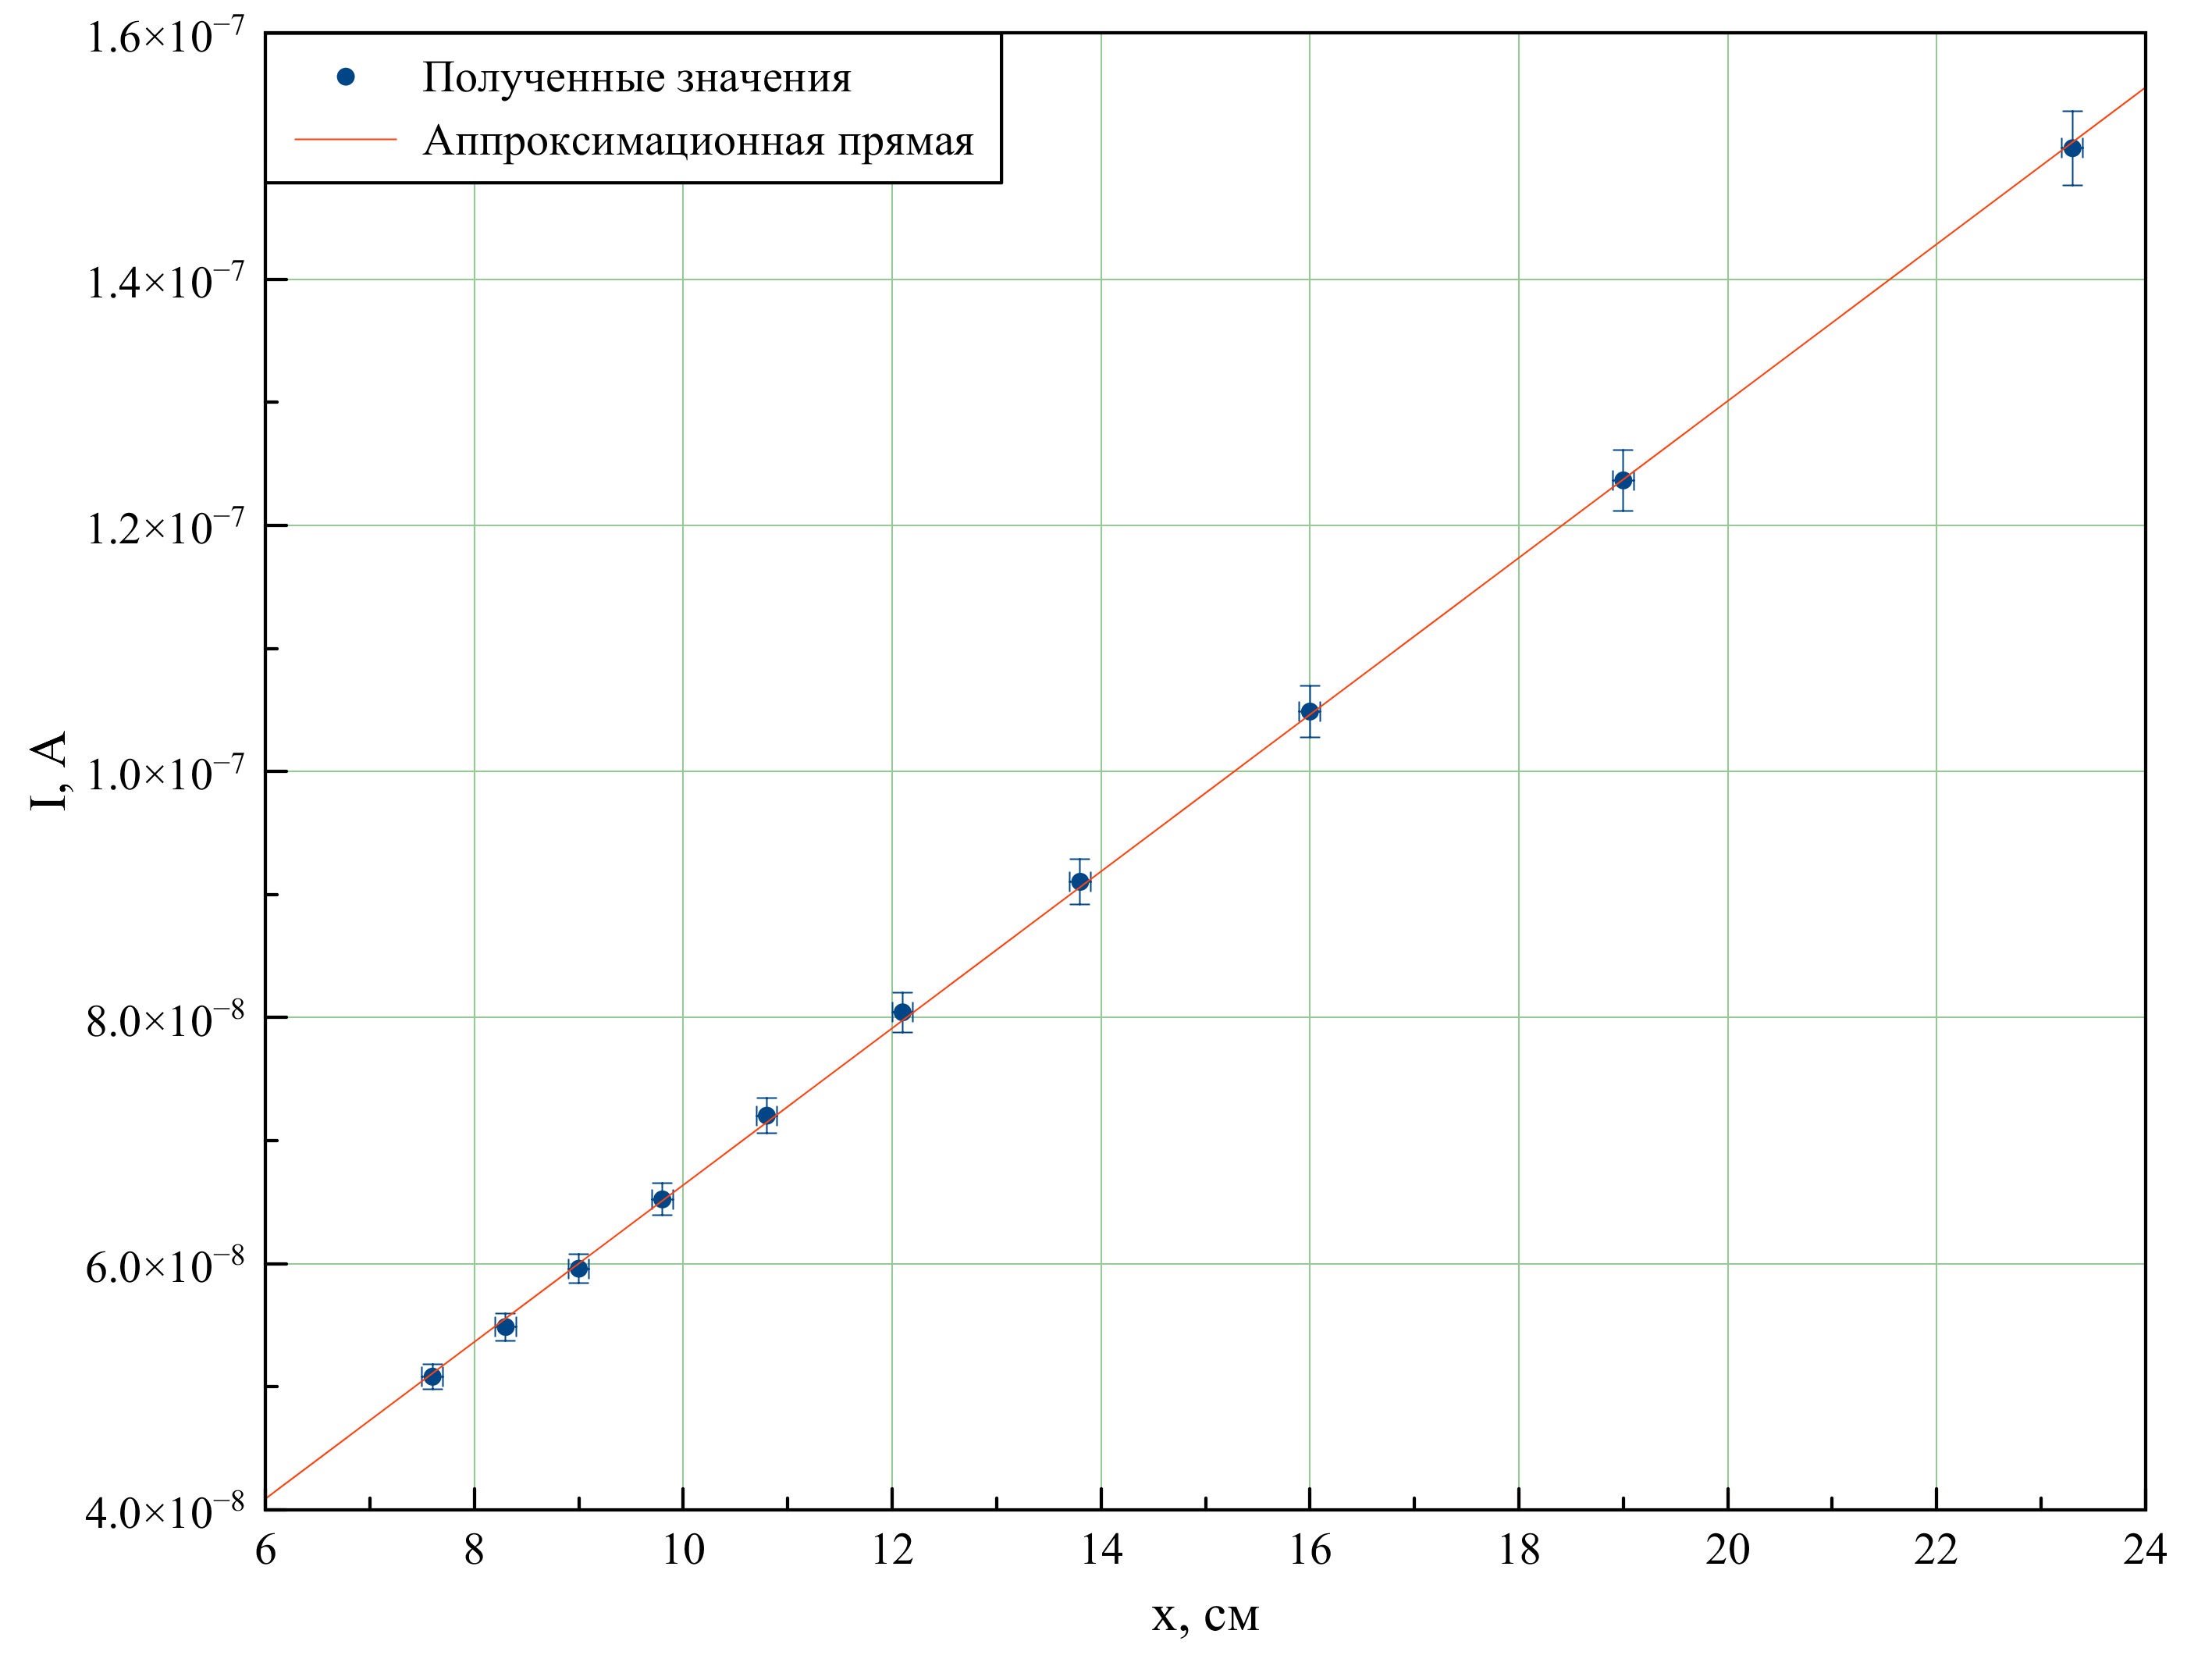
\includegraphics[width = 0.9\linewidth]{grph1}
	\caption[h]{График зависимости $I=f(x).$}
\end{figure}

С помощью метода наименьших квадратов определим угловой коэффициент наклона аппроксимационной прямой:
$$k =\dfrac{<x\cdot I>}{<x^2>} \simeq 6.55 \cdot 10^{-7}~\text{А/м} = 6.56 \cdot 10^{-10}~\text{А/мм}$$
$$\sigma_k = \dfrac{1}{\sqrt{10}}\cdot \sqrt{\dfrac{<I^2>}{<x^2>} - k^2} \simeq 2.36 \cdot 10^{-9}~\text{А/м} = 2.36\cdot 10^{-12}~\text{А/мм}.$$

По наклону прямой рассчитаем динамическую постоянную $C_I$ по формуле (\ref{f15}):
$$C_I = \dfrac{2aI}{x} \simeq 1.44 \cdot 10^{-9}~\frac{\text{А}}{\text{мм/м}}. $$

Окончательно получаем:
$$
\fbox{\text{$C_I \simeq (1.44 \pm 0.01)\cdot 10^{-9}~\frac{\text{А}}{\text{мм/м}}~(\varepsilon \simeq 0.4\%)$}}
$$

\subsection{Определение критического сопротивления.}

Измерим два последовательных отклонения зайчика в одну сторону ($ x_n = 21.3~\text{см},~ x_{n+1} \hm{=} 19.4~\text{см}$). Рассчитаем логарифмический декремент затухания $\Theta_0$ разомкнутого гальванометра по формуле (\ref{eq:theta}):
$$\Theta_0 = \ln\dfrac{x_n}{x_{n+1}} \simeq 0.09$$

Построим график $1/\Theta^2 = f[(R+R_0)^2]$ и по наклону прямой(в области малых $R$) рассчитаем критическое сопротивление по формуле (\ref{f21}).

\begin{table}[H]
	\centering
	\caption{Определение критического сопротивления.}
	\label{t2}
	\begin{tabular}{c|ccccccc}
		\toprule
		$x_n,~\text{см}$                   & 5.7  & 10.5 & 9.8   & 17.7  & 16.4  & 15.4  & 14.5  \\
		$x_{n+1},~\text{см}$               & 1.0    & 2.7  & 3.2   & 6.4   & 6.6   & 6.7   & 6.8   \\
		$\Theta$                           & 1.74 & 1.36 & 1.12  & 1.02  & 0.91  & 0.83  & 0.76  \\
		$R+R_0,~\text{Ом}$                 & 7080 & 8780 & 10480 & 12180 & 13880 & 15580 & 17280 \\ \midrule
		$(R+R_0)^2\cdot 10^8,~\text{Ом}^2$ & 0.50 & 0.77 & 1.09  & 1.48  & 1.93  & 2.43  & 2.99  \\
		$1/\Theta^2$                       & 0.33 & 0.54 & 0.79  & 0.97  & 1.21  & 1.44  & 1.74 \\ \bottomrule
	\end{tabular}
\end{table}

\begin{figure}[H]
	\centering
	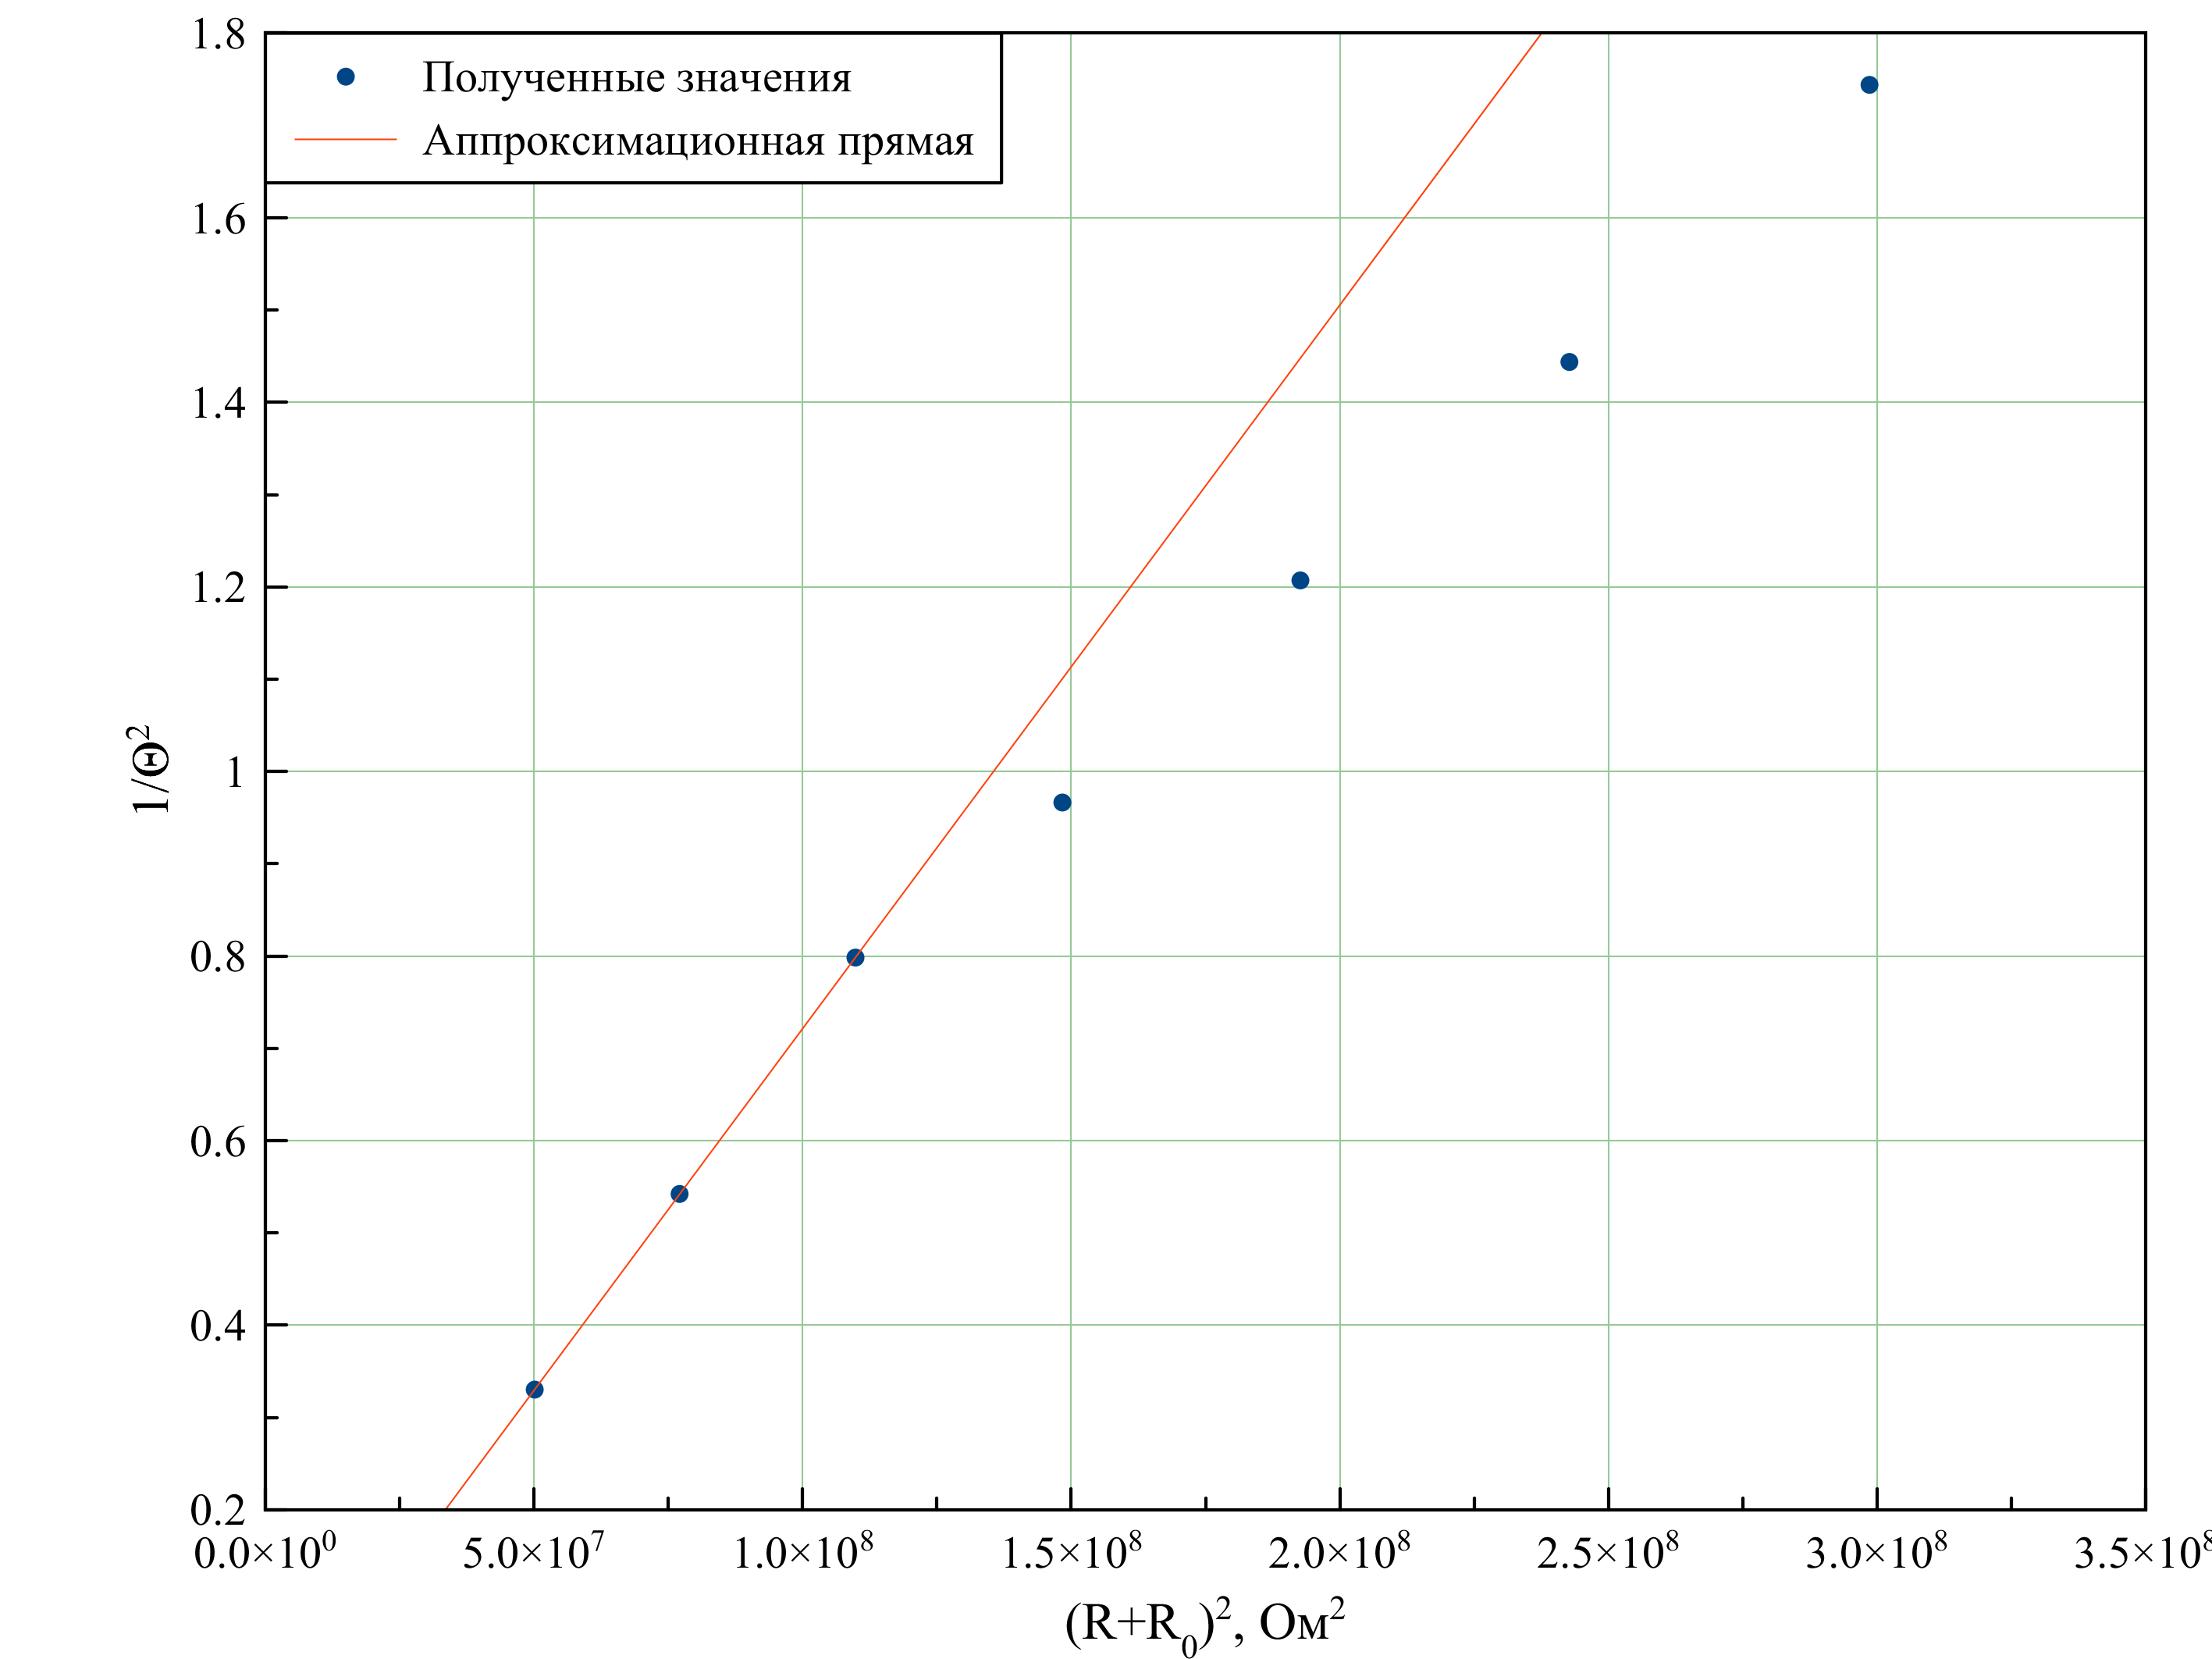
\includegraphics[width = 0.8\linewidth]{grph2}
	\caption[h]{График зависимости $1/\Theta^2=f[(R+R_0)^2].$}
\end{figure}

С помощью метода наименьших квадратов определим тангенс угла наклона аппроксимационной прямой:
$$k = \dfrac{<1/\Theta^2\cdot (R+R_0)^2>-<(R+R_0)^2><1/\Theta^2>}{<(R+R_0)^4>-<(R+R_0)^2>^2} \simeq 7.84\cdot 10^{-9}~\text{Ом}^{-2} $$
$$\sigma_k = \dfrac{1}{\sqrt{3}}\cdot \sqrt{\dfrac{<1/\Theta^4>-<1/\Theta^2>^2}{<(R+R_0)^4> - <(R+R_0)^2>^2} -k^2} \simeq 6.8\cdot 10^{-12}~\text{Ом}^{-2}$$

$$R_{\text{кр}} = \dfrac{1}{2\pi}\sqrt{\dfrac{\Delta X}{\Delta Y}}-R_0 \simeq 1518~\text{Ом}$$
Окончательно получаем:
\begin{equation*}
\fbox{\text{$
R_{\text{кр}} \simeq (1518 \pm 1)~\text{Ом}~(\varepsilon \simeq 0.1\% )$}}
\end{equation*}

Перейдём к изучению гальванометра в баллистическом режиме. Построим график $l_{\text{max}} = f[(R+R_0)^{-1}]$. Определим по графику критическое сопротивление гальванометра (с учётом (\ref{f23})).

\begin{table}[H]
	\centering
	\caption{Таблица зависимости $l_{max}[(R_0+R)^{-1}]$}
	\label{my-label}
	\resizebox{\textwidth}{!}{
	\begin{tabular}{c|ccccccccccccccc}\toprule
		$R,~\text{кОм}$                           & 0.09    & 0.5   & 0.6   & 0.70   & 0.8  & 0.9  & 1 & 2 & 5 & 8 & 10 & 20 & 30 & 40 & 50 \\ \midrule
		$\frac{1}{(R+R_0)}\cdot 10^{-5},~\text{Ом}^{-1}$ & 270.3 & 128.2 & 113.6 & 102.0 & 92.6 & 84.7 & 78.1 & 43.9 & 18.9 & 12.1 & 9.7   & 4.9   & 3.3   & 2.5   & 1.9   \\
		$l_{max},~\text{см}$                     & 2.3   & 4.5   & 4.7   & 5.1   & 5.4  & 5.7  & 6.2  & 8.5  & 12.2 & 14.2 & 14.7  & 16.6  & 17.2  & 17.5  & 17.8 \\ \bottomrule
	\end{tabular}
}
\end{table}

\begin{figure}[H]
	\centering
	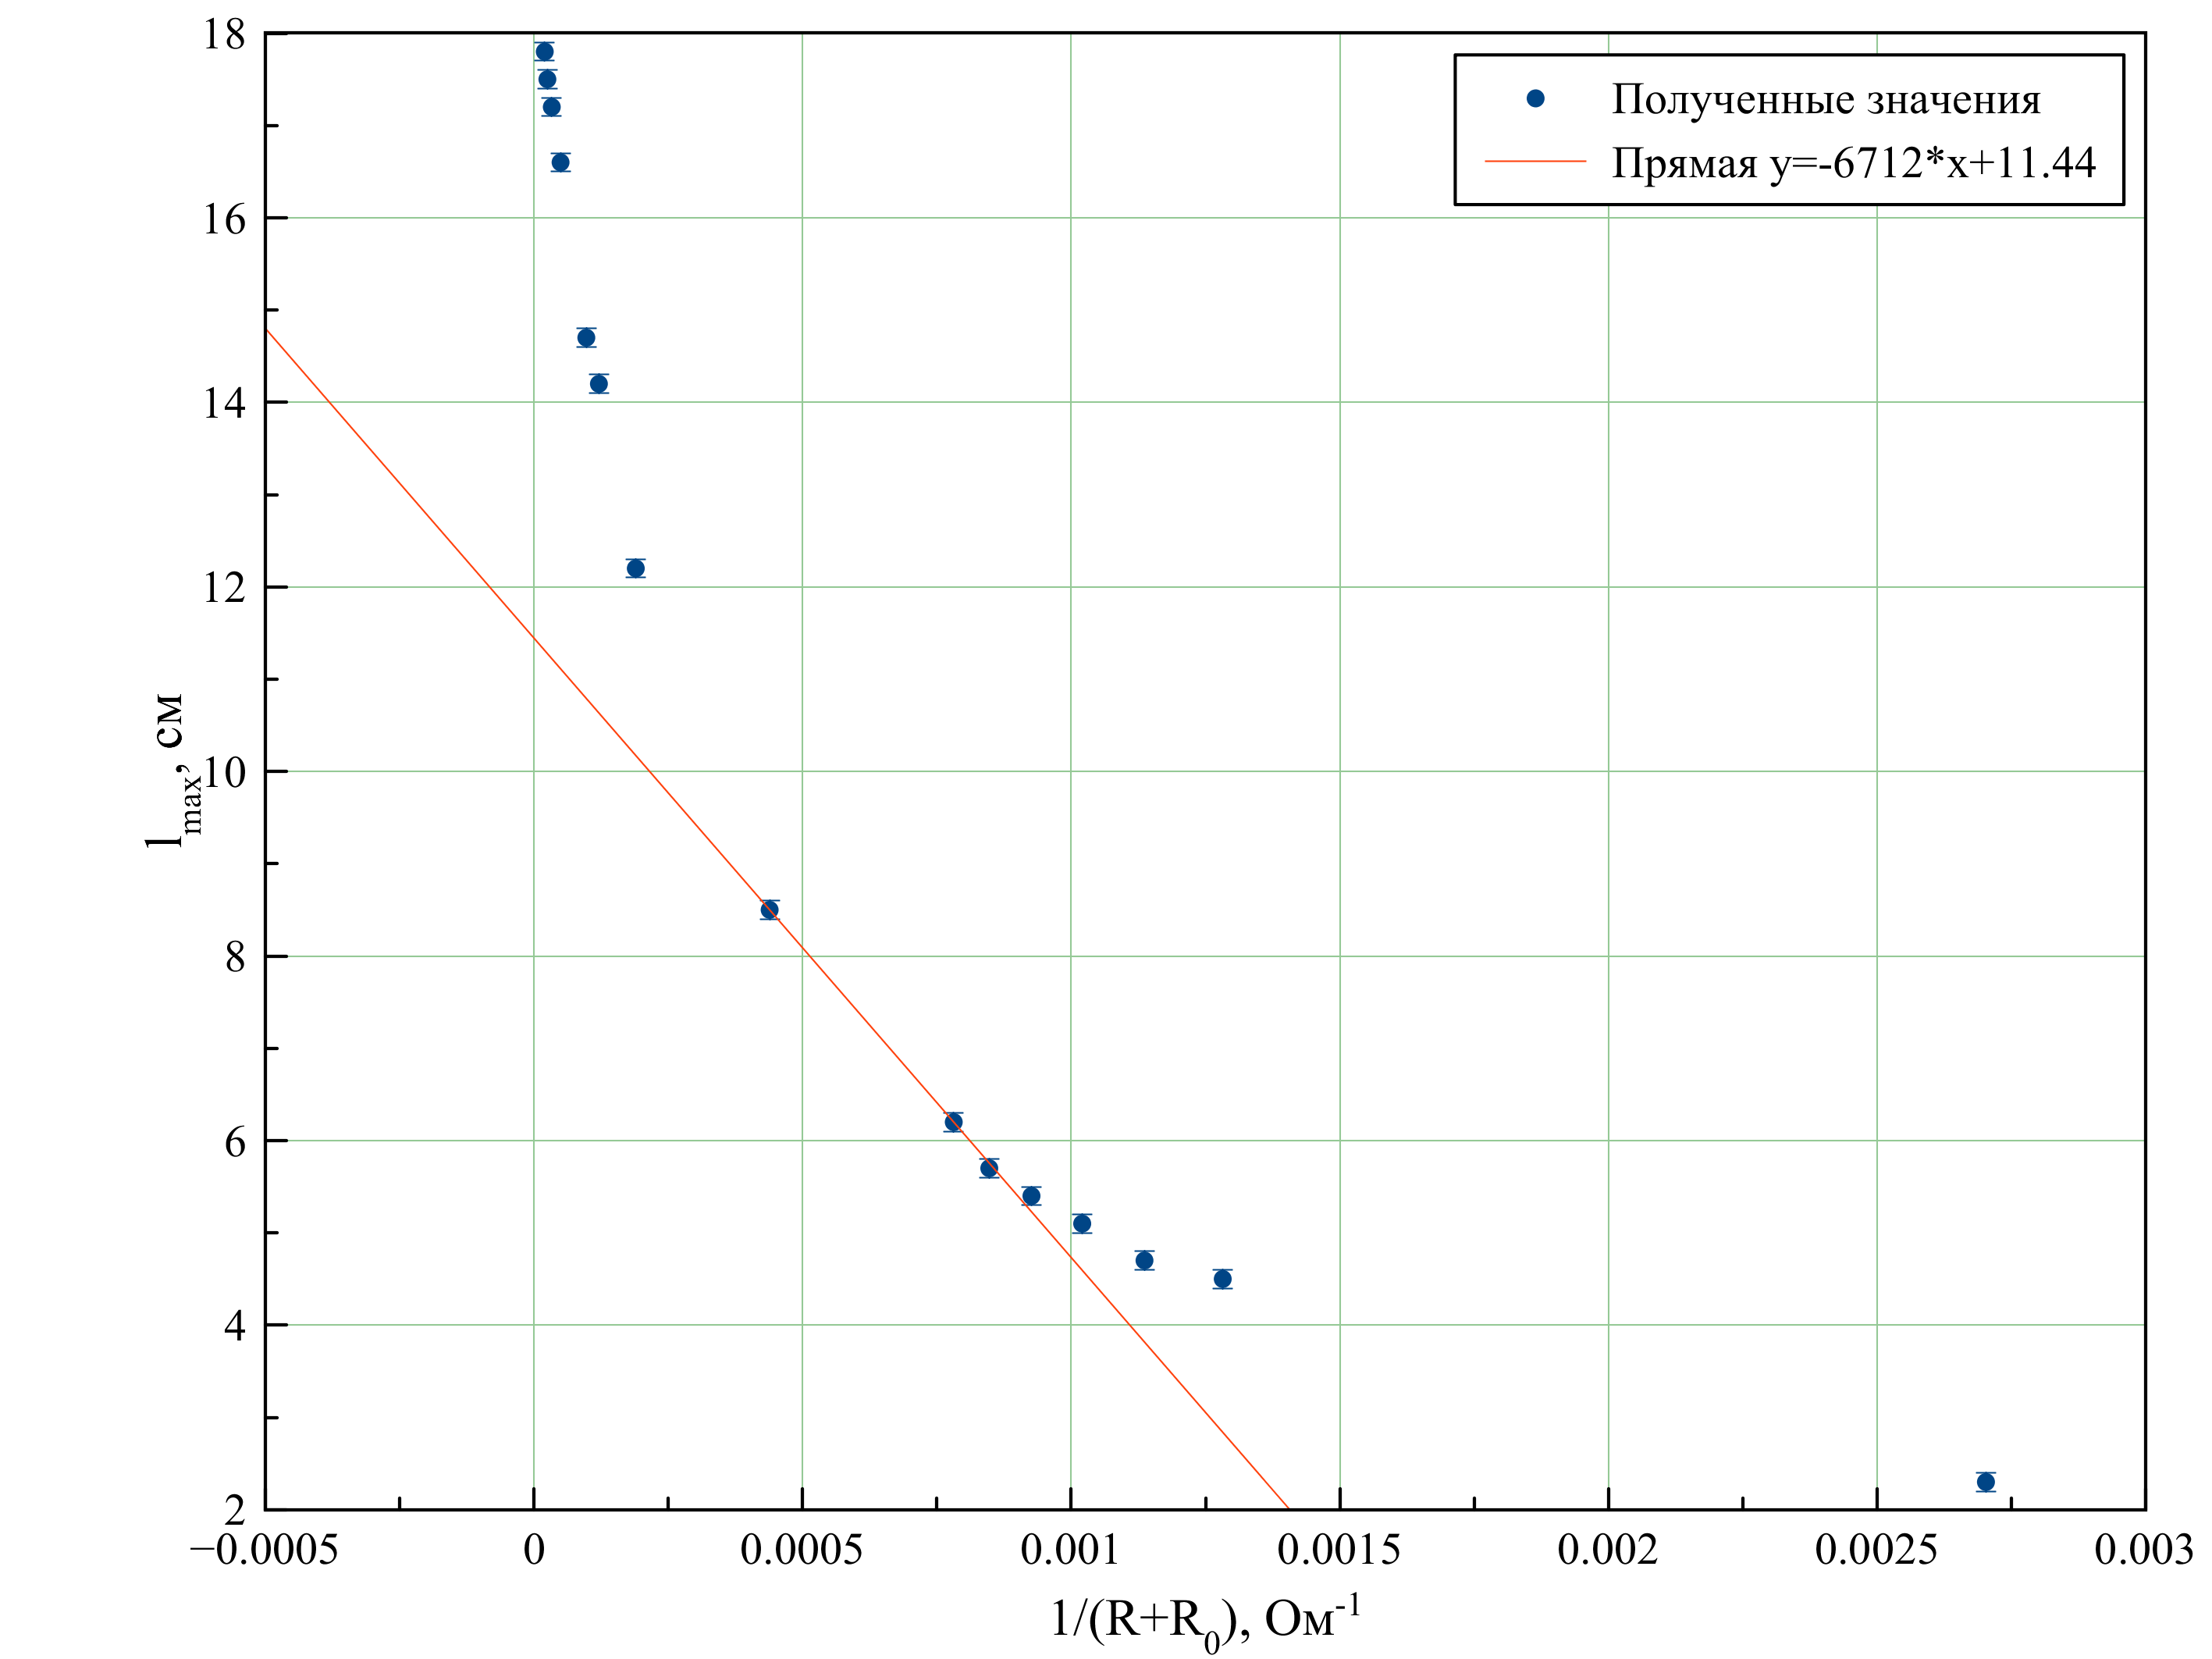
\includegraphics[width = 0.9\linewidth]{grph3}
	\caption[h]{График зависимости $l_{max} = f[(R+R_0)^{-1}]$.}
\end{figure}

Сравним значения $R_{\text{кр}}$, измеренные различными способами (см. таблицу (\ref{t3})).

\begin{table}[H]
	\centering
	\caption{Значения $R_{\text{кр}}$.}
	\label{t3}
	\begin{tabular}{c|ccc} \toprule
		Способ                     & Эксперимент & \begin{tabular}[c]{@{}c@{}}Стационарный\\ режим\end{tabular} & \begin{tabular}[c]{@{}c@{}}Баллистический \\  режим\end{tabular} \\ \midrule
		$R_{\text{кр}},~\text{Ом}$ & $1700$      & $1518 \pm 1$                                                 & $1284$     \\ \bottomrule                                                    
	\end{tabular}
\end{table}

\subsection{Определение баллистической постоянной.}

Рассчитаем баллистическую постоянную в критическом режиме $C_{Q_{\text{ кр}}}$ по формуле (\ref{f24}):
$$C_{Q_{\text{ кр}}} = 2a\dfrac{R_1}{R_2}\dfrac{U_0C}{l_{max_{\text{ кр}}}} \simeq 2.08\cdot 10^{-9}~[\text{К/(мм/м)}]$$

С учётом погрешности получаем:
\begin{equation*}
\fbox{\text{$C_{Q_{\text{ кр}}} \simeq (2.08 \pm 0.03) \cdot 10^{-9}~[\text{К/(мм/м)}] (\varepsilon \simeq 1.4 \%) $}}
\end{equation*}

Сравним время релаксации $t$ и период свободных колебаний гальванометра $T_0$:
$$t = R_0C \simeq 280*2\cdot 10^{-6} \simeq 5.6\cdot 10^{-4}~\text{с}$$
$$T_0 = \dfrac{T}{n} \simeq \dfrac{74.6}{10} \simeq 7.5~\text{с}$$

\section{Вывод.}
В данной лабораторной работе мы измерили значение динамической постоянной гальванометра, критического сопротивления тремя способами и баллистической постоянной. В измерениях динамической постоянной значения $R_\text{кр}$ близки, но все же не совпадают (это можно объяснить тем, что экспериментальное значение $R_{\text{кр}}$ измерено с большой погрешностью, так как оно определялось на "глаз"). Наибольшая погрешность в третьем эксперименте, так как большой вклад в погрешность даёт скорость реакции человека (отклонения зайчика происходят быстро, необходимо успевать замыкать ключ и считывать значения).





\end{document}

